\chapter{Metodología de diseño e implementación de recursos distribuidos}
\label{cap:metodologia}


Una vez que el modelado se ha completado es tiempo de abarcar la metodología que se sigue a la hora de diseñar e implementar nuevos recursos distribuidos. Para ello se usan las facilidades que proporciona la herramienta de gestión de configuración para ampliar su funcionalidad.


%%%%%%%%%%%%%%%%%%%%%%%%%%%%%%%%%%%%%%%%%%%%%%%%%%%%%%%%%%%%%%%%%%%%%%%%%%%%%%%%
\section{Especificación del tipo}

El primer paso que hay que hacer a la hora de crear un nuevo recurso en Puppet es definir el tipo de recurso. Para ello en un fichero habrá que especificar el nombre del nuevo tipo y los argumentos que éste tiene. Durante esta sección y la siguiente se usará el ejemplo de la arquitectura web de tres niveles ya que es la más conocida y sirve para demostrar que el enfoque que se ha tomado es lo suficientemente general y válido también para infraestructuras que nada tienen que ver con la ejecución de trabajos. \\

Una típica arquitectura de servicios web consta de al menos tres niveles: balanceo de carga, servidores web y base de datos. Cada uno de estos niveles está compuesto por al menos un elemento clave: el balanceador de carga, el servidor web y el servidor de base de datos, respectivamente. El balanceador de carga es el punto de entrada al sistema y el que se encarga, como su nombre indica, de repartir las peticiones de los clientes a los distintos servidores web. Los servidores web se encargan de servir las páginas web a los clientes y para ello, dependiendo de las peticiones que hagan los clientes, podrán leer o almacenar información en la base de datos. Para manipular dicha información los servidores web tendrán que comunicarse con el servidor de base de datos, que es el que hará efectiva la lectura y modificación de la información.\\

\begin{figure} [!htbp]
  \centering
  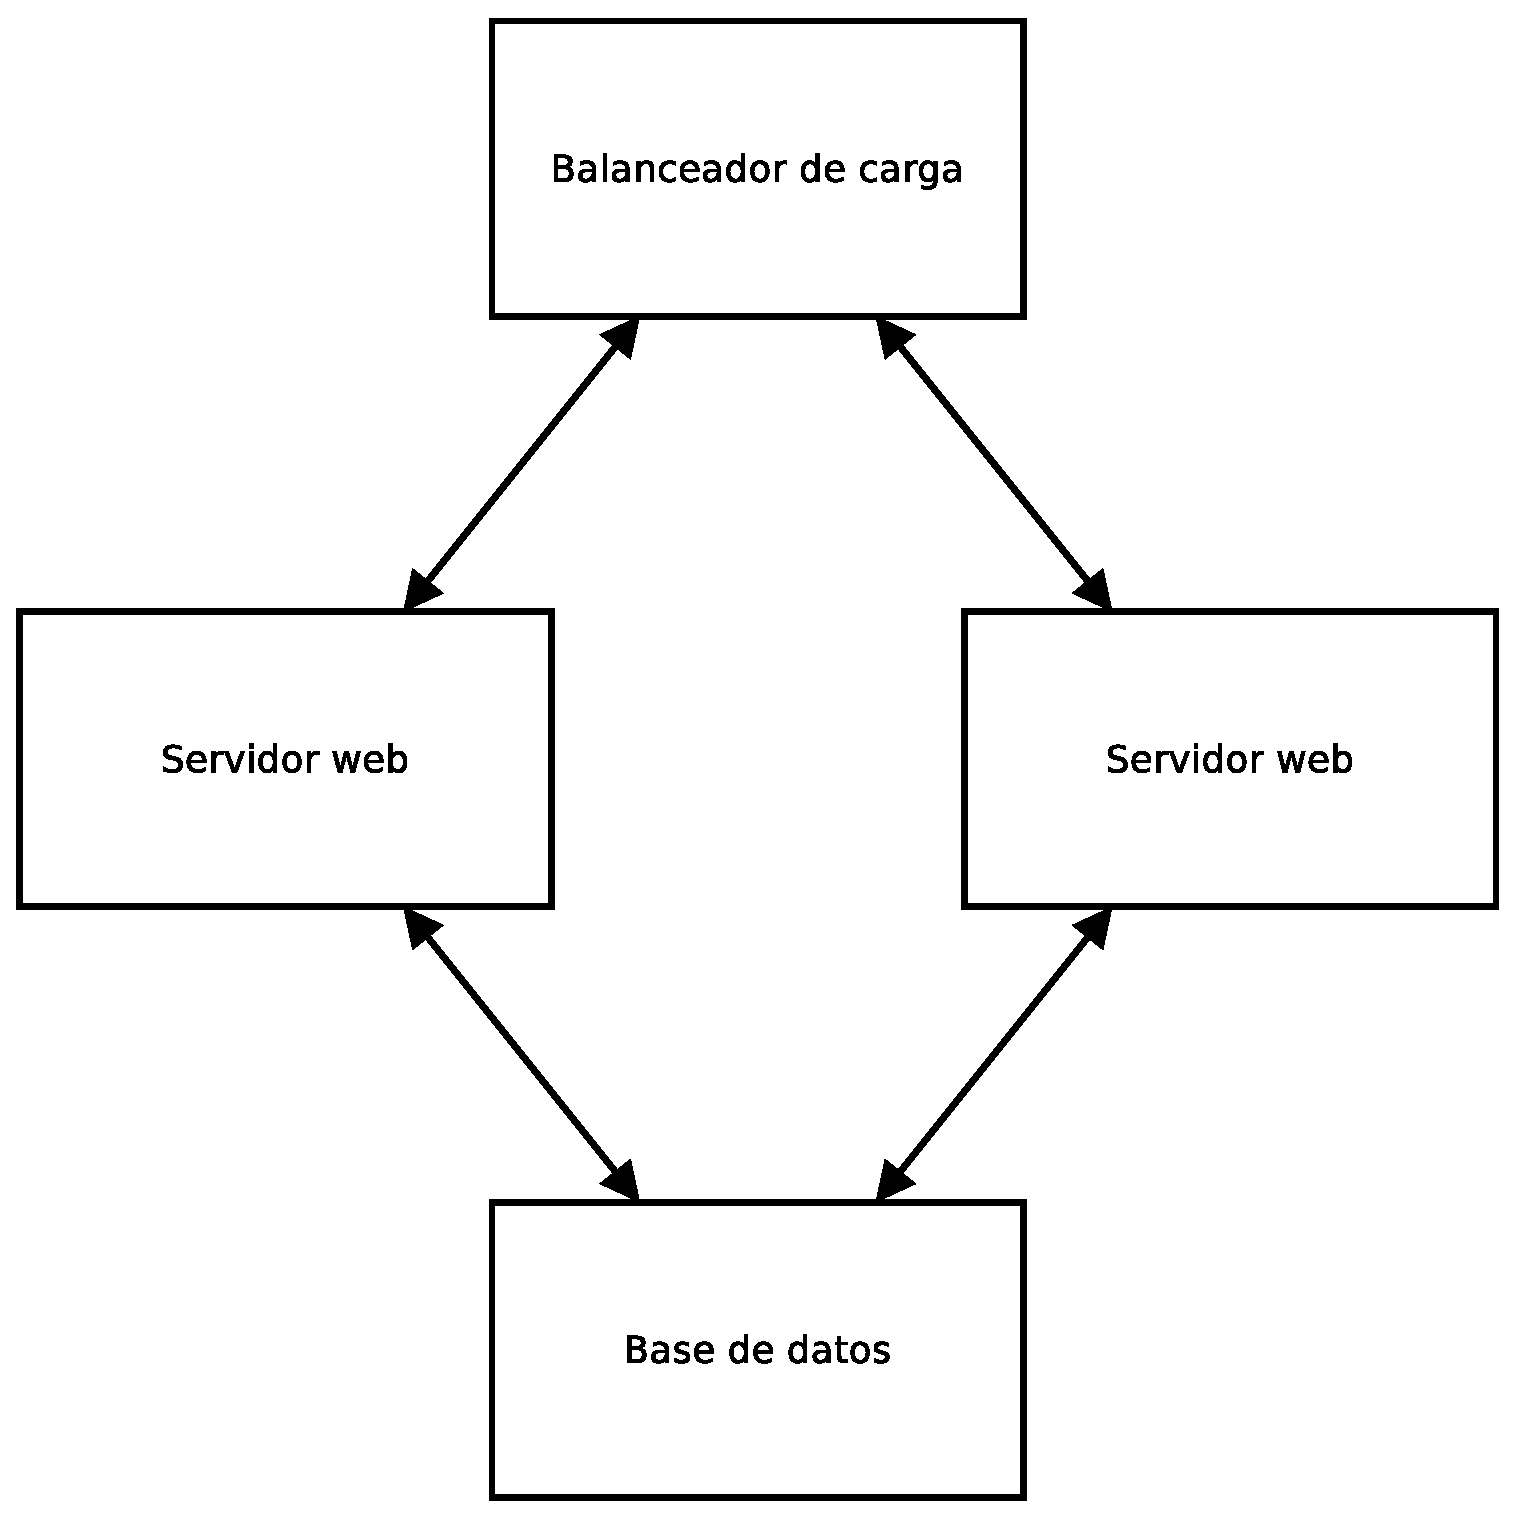
\includegraphics[width=0.5\textwidth]{figuras/Arquitectura_Web2.eps}
  \caption{Infraestructura web de tres niveles.}
\label{figure:arquitectura-web}
\end{figure}

La infraestructura usada como ejemplo consta de un balanceador de carga, dos servidores web y un servidor de bases de datos (Figura \ref{figure:arquitectura-web}).


\pagebreak

La creación del tipo \texttt{web} se hace en el fichero \texttt{web.rb}, en el lugar apropiado dentro del correspondiente módulo. En el siguiente fragmento de código se indican los aspectos más importantes del mismo (la implementación completa puede encontrarse en el Anexo \ref{anx:codigo}):

\begin{rubycode}
Puppet::Type.newtype(:web) do
   @doc = "Manages web clouds formed by KVM virtual machines."
   
   
   ensurable do

      desc "The cloud's ensure field can assume one of the following values:
   `running`: The cloud is running.
   `stopped`: The cloud is stopped.\n"
   
      newvalue(:stopped) do
         provider.stop
      end

      newvalue(:running) do
         provider.start
      end

   end


   # General parameters
   
   newparam(:name) do
      desc "The cloud name"
      isnamevar
   end
   
   newparam(:vm_domain) do
      desc "The XML file with the virtual machine domain definition. " +
           "Libvirt XML format must be used"
   end
   
   newproperty(:pool, :array_matching => :all) do
      desc "The pool of physical machines"
   end

   # ...


   # Web parameters
   
   newproperty(:balancer, :array_matching => :all) do
      desc "The balancer node's information"
   end
   
   newproperty(:server, :array_matching => :all) do
      desc "The server nodes' information"
   end
   
   newproperty(:database, :array_matching => :all) do
      desc "The database node's information"
   end

end

\end{rubycode}

Dentro del tipo \texttt{web}, los atributos \texttt{name}, \texttt{vm\_domain} y \texttt{pool} se corresponden con los atributos \texttt{Nombre}, \texttt{Fichero de dominio} y \texttt{Conjunto de máquinas físicas} definidos en la sección \ref{sec:modelado-puppet}. Los atributos \texttt{balancer}, \texttt{server} y \texttt{database} son los atributos propios de la arquitectura web.

Una vez que el tipo está definido, ya se puede ver cuál será el aspecto de un manifiesto para un recurso de tipo web:


\begin{lstlisting}
web {'mycloud':
   balancer  => ["155.210.155.175", "/var/tmp/dceresuela/lucid-lb.img"],
   server    => ["/etc/puppet/modules/web/files/server-ips.txt",
                 "/etc/puppet/modules/web/files/server-imgs.txt"],
   database  => ["155.210.155.177", "/var/tmp/dceresuela/lucid-db.img"],
   vm_domain => "/etc/puppet/modules/web/files/mycloud-template.xml",
   pool      => ["155.210.155.70"],
   ensure    => running,
}
\end{lstlisting}

%%%%%%%%%%%%%%%%%%%%%%%%%%%%%%%%%%%%%%%%%%%%%%%%%%%%%%%%%%%%%%%%%%%%%%%%%%%%%%%%
\section{Diseño e implementación del proveedor}

Después de haber definido el tipo del recurso, queda definir el proveedor que implementa dicho tipo. En el caso de los recursos distribuidos, y teniendo en cuenta las funciones de arranque y parada especificadas en el tipo (en el bloque \texttt{ensurable}, líneas 5 a 19), el proveedor deberá contener obligatoriamente las funciones \texttt{start} y \texttt{stop}. A continuación se presenta un proveedor con los aspectos más importantes (la implementación completa se encuentra en el Anexo \ref{anx:codigo}):

\begin{rubycode}
Puppet::Type.type(:web).provide(:webp) do
   desc "Manages web clouds formed by KVM virtual machines"

   # Require files
   # ...

   # Start function. Makes sure the cloud is running.
   def start
   
      cloud = Cloud.new(CloudInfrastructure.new(), CloudLeader.new(), resource,
                        method(:err))
      puts "Starting cloud %s" % [resource[:name]]
      
      # Check existence
      if !exists?
         # Cloud does not exist => Startup operations
         
         # Check pool of physical machines
         puts "Checking pool of physical machines..."
         pm_up, pm_down = cloud.check_pool()
         unless pm_down.empty?
            puts "Some physical machines are down"
            pm_down.each do |pm|
               puts " - #{pm}"
            end
         end
         
         # Obtain the virtual machines' IPs
         puts "Obtaining the virtual machines' IPs..."
         vm_ips, vm_ip_roles, vm_img_roles = obtain_vm_data(cloud.resource)
         
         # Check whether you are one of the virtual machines
         puts "Checking whether this machine is part of the cloud..."
         part_of_cloud = vm_ips.include?(MY_IP)
         if part_of_cloud
            puts "#{MY_IP} is part of the cloud"
            
            # Check if you are the leader
            if cloud.leader?()
               cloud.leader_start("web", vm_ips, vm_ip_roles, vm_img_roles,
                                  pm_up, method(:web_monitor))
            else
               cloud.common_start()
            end
         else
            puts "#{MY_IP} is not part of the cloud"
            cloud.not_cloud_start("web", vm_ips, vm_ip_roles, vm_img_roles,
                                  pm_up)
         end
         
      else
         
         # Cloud exists => Monitoring operations
         puts "Cloud already started"
         
         # Check if you are the leader
         if cloud.leader?()
            cloud.leader_monitoring(method(:web_monitor))
         else
            puts "#{MY_IP} is not the leader"      # Nothing to do
         end
      end
      
   end


   # Stop function. Makes sure the cloud is not running.
   def stop

      # ...
   
   end


   def status
      if File.exists?("/tmp/cloud-#{resource[:name]}")
         return :running
      else
         return :stopped
      end
   end
   
end
\end{rubycode}

Son especialmente importantes dentro de este proveedor las líneas 10, 30 y 40. En la línea 10 creamos un nuevo objeto de la clase \texttt{Cloud} (\ref{sec:modelado-framework}). En la línea 30 se llama a la función \texttt{obtain\_vm\_data} para obtener los datos de las máquinas virtuales (\ref{sec:modelado-framework}). En la línea 40 puede verse como el objeto de la clase \texttt{Cloud} se usa para llamar al método \texttt{leader\_start} que realizará las funciones de puesta en marcha como nodo líder del \emph{cloud} (\ref{sec:modelado-proveedor}). Uno de los argumentos del método en esa llamada es la función \texttt{web\_monitor} que se usará para monitorizar los aspectos particulares del \emph{cloud} web (\ref{sec:modelado-framework}). \\

Merece la pena comentar que tanto para la implementación del tipo como para la del proveedor Puppet hace uso de la capacidad de metaprogramación que ofrece Ruby. La implementación de cada uno de ellos se pasa como un bloque de código Ruby a una función de Puppet (\texttt{newtype} para el tipo y \texttt{provide} para el proveedor) que se encarga internamente de realizar las operaciones necesarias. Es por este motivo que en el código del tipo y del proveedor aparecen variables (como \texttt{resource} y \texttt{provider}) y funciones (como \texttt{newparam} y \texttt{desc}) que no pertenecen a la sintaxis del lenguaje Ruby y no se encuentran \emph{a priori} definidas en ninguna parte. Gracias a la ejecución dinámica de Ruby sabemos que estas variables y funciones estarán definidas en el entorno de Puppet en tiempo de ejecución.
